\chapter{FtsZ: function and structure}\label{ftsz}

To better understand the role of FtsZ in the septation of \textit{D. radiodurans}, we investigated its structure and superstructure using both single particle cryo-EM and \textit{in situ} cryo-ET.
This work is ongoing and not yet consolidated into a manuscript for publication.
Sample preparation and screening was performed by my supervisors Irina Gutsche and Joanna Timmins, while data collections were done partly by Irina, and partly commissioned to external facilities.
Data processing on the single particle and tomography data, and software tool development were performed by me, and progressively handed off to Harald Bernhard, a postdoc in the MICA group.

\localtableofcontents

\section{State of the art}

FtsZ is an extremely well conserved prokaryotic tubulin homologue, known to form ring-like structures (the Z-ring) at the septation site in most bacteria.
It polymerizes in a GTP-dependent fashion to form filaments and bundles, anchoring to the membrane via its partner FtsA, and interacting with several other partners in the cytokinesis and peptidoglycan (PG) synthesis machinery~\cite{barrowsFtsZDynamicsBacterial2021,mcquillenInsightsStructureFunction2020}.

Based on crystal structures, filaments have been shown to form through head-to-tail stacking of monomers CITE.
However, there is no structural information regarding the flexible C-terminal region, which is responsible for regulating its activity and interaction with its cellular partners, including FtsA.
It's also unclear how multiple filaments may assemble to form bundles at the structural level and even less so in vivo.
Thus --- while its key role in cell division is undisputed --- the exact mechanism and function of FtsZ are still unclear.
There is currently no consensus model that fully explains the function and mode of action of FtsZ in the division process in bacteria, as the current evidence is inconclusive, sometimes presenting significant variations between species --- likely ascribable to different shapes or membrane compositions between bacteria~\cite{barrowsFtsZDynamicsBacterial2021,mcquillenInsightsStructureFunction2020}.

\begin{figure}[ht]
    \centering
    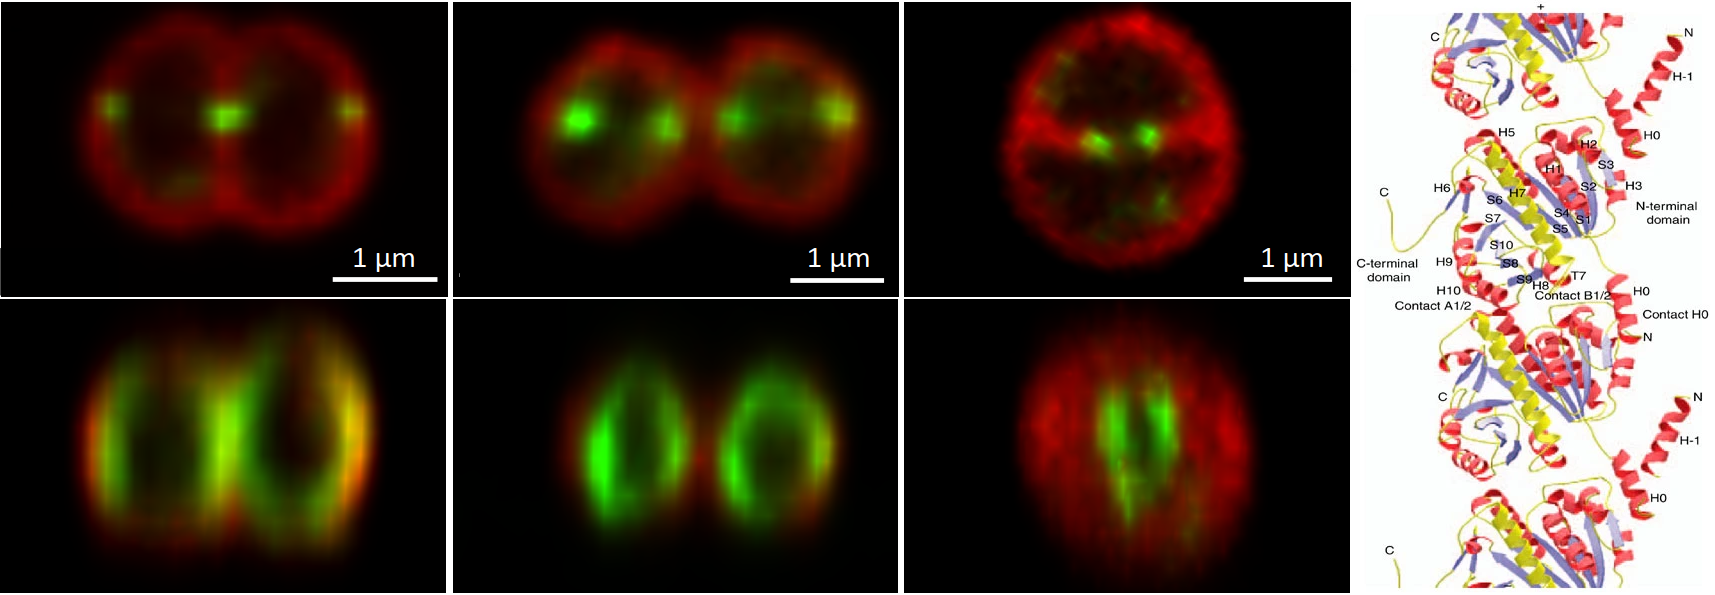
\includegraphics[width=.5\textwidth]{other/ftsz_ring.png}
    \titledcaption[FtsZ forms a ring \textit{in vivo} and filaments \textit{in vitro}]{During cell division, FtsZ is known to localize on a ring (termed Z-ring) corresponding to the tips of the septa (left, figure adapted from \autoref{drad_fig6}). Many structural studies were done on FtsZ, identifying the formation of protofilament via head-to-tail stacking (right, figure adapted from \citet{olivaStructuralInsightsFtsZ2004}.}
    \label{fig:ftsz_ring}
\end{figure}

Some studies have shown that FtsZ presents mechanical functions that may drive the septation process.
\textit{T. maritima} FtsZ+FtsA expressed in liposomes was shown to form coil-like structures, which can constrict the membrane via a "filament sliding" mechanism, creating a partial septum~\cite{szwedziakArchitectureRingFormed2014}.
In \textit{C. crescentus}, FtsZ may form short, loosely bundled filaments, which may drive constriction via an "iterative pinching" mechanism where repeated rounds of phosphorylation lightly bend the filament, thus slowly pinching the membrane~\cite{liStructureFtsZFilaments2007}.

Other publications investigated the recruitment and signalling role of FtsZ for downstream machinery such as PG synthesis.
FtsZ was shown to undergo plus-end polymerization and minus-end depolymerization, in a GTP-regulated process typical of cytoskeletal proteins called treadmilling~\cite{looseBacterialCellDivision2014}.
In \textit{B. subtilis}, this treadmilling is required to drive the movement along the septum of the PG synthesis centers~\cite{bisson-filhoTreadmillingFtsZFilaments2017}.
A "diffusion-and-capture" model was proposed, where the FtsZ ring performs a recruitment role by engaging in weak transient interactions with downstream machinery for PG synthesis~\cite{baranovaDiffusionCapturePermits2020}.
However, in \textit{S. aureus}, cytokinesis may actually occur in two separate steps: a slow, FtsZ-driven, treadmilling-dependent step which causes initial invagination, followed by a faster step where PG synthesis is the driving force for septation~\cite{monteiroPeptidoglycanSynthesisDrives2018}.

While FtsZ ring formation and PG synthesis are clearly linked, their precise interaction may differ between bacteria.
In \textit{E. coli}, GTP regulates FtsZ treadmilling, which in turn controls the movement of the synthesis machinery~\cite{yangGTPaseActivityCoupled2017}.
However, it does not appear to affect the rate of PG synthesis, as opposed to what happens in \textit{B. subtilis}, which suggest that the presence or absence of an outer membrane may change PG synthesis machinery regulation~\cite{yangGTPaseActivityCoupled2017}.
Indeed, in \textit{E. coli}, some additional proteins may help with a timely invagination of the outer membrane, although they are not needed for septation to occur~\cite{gerdingTransenvelopeTolPal2007}.
This is intriguing for \textit{D. radiodurans} which, despite staining gram-positive, presents an outer membrane.

The disordered C-terminal domain of FtsZ was found to be necessary both for the anchorage to the membrane via FtsA, and to regulate oligomerization as well as bundling with neighboring filaments~\cite{barrowsFtsZDynamicsBacterial2021}.

Collectively, the literature hints that FtsZ treadmilling is likely not the only factor that controls the dynamics of FtsZ and the Z-ring, and that variations across species may be explained by different divergent mechanisms, or some other underlying behavior not yet discovered~\cite{barrowsFtsZDynamicsBacterial2021}.

\section{Structural study by SPA}

We began our investigation of the structure of DrFtsZ filaments by doing SPA on \textit{in vitro} samples prepared with purified monomeric FtsZ from \textit{D. radiodurans}.
Since successful polymerization is highly sensitive to FtsZ concentration, temperature, concentration of GTP (or other nucleotide), and elongation time, my supervisors tested a variety of conditions, using both negative stain EM and cryo-EM for screening.
The selected preparation(\fullref{ftsz_methods}) resulted in FtsZ filaments long enough to allow filament picking and helical reconstruction, while avoiding an excess of filament bundles which make picking and refinement more difficult (\autoref{fig:ftsz_micrographs}).

\begin{figure}[ht]
    \centering
    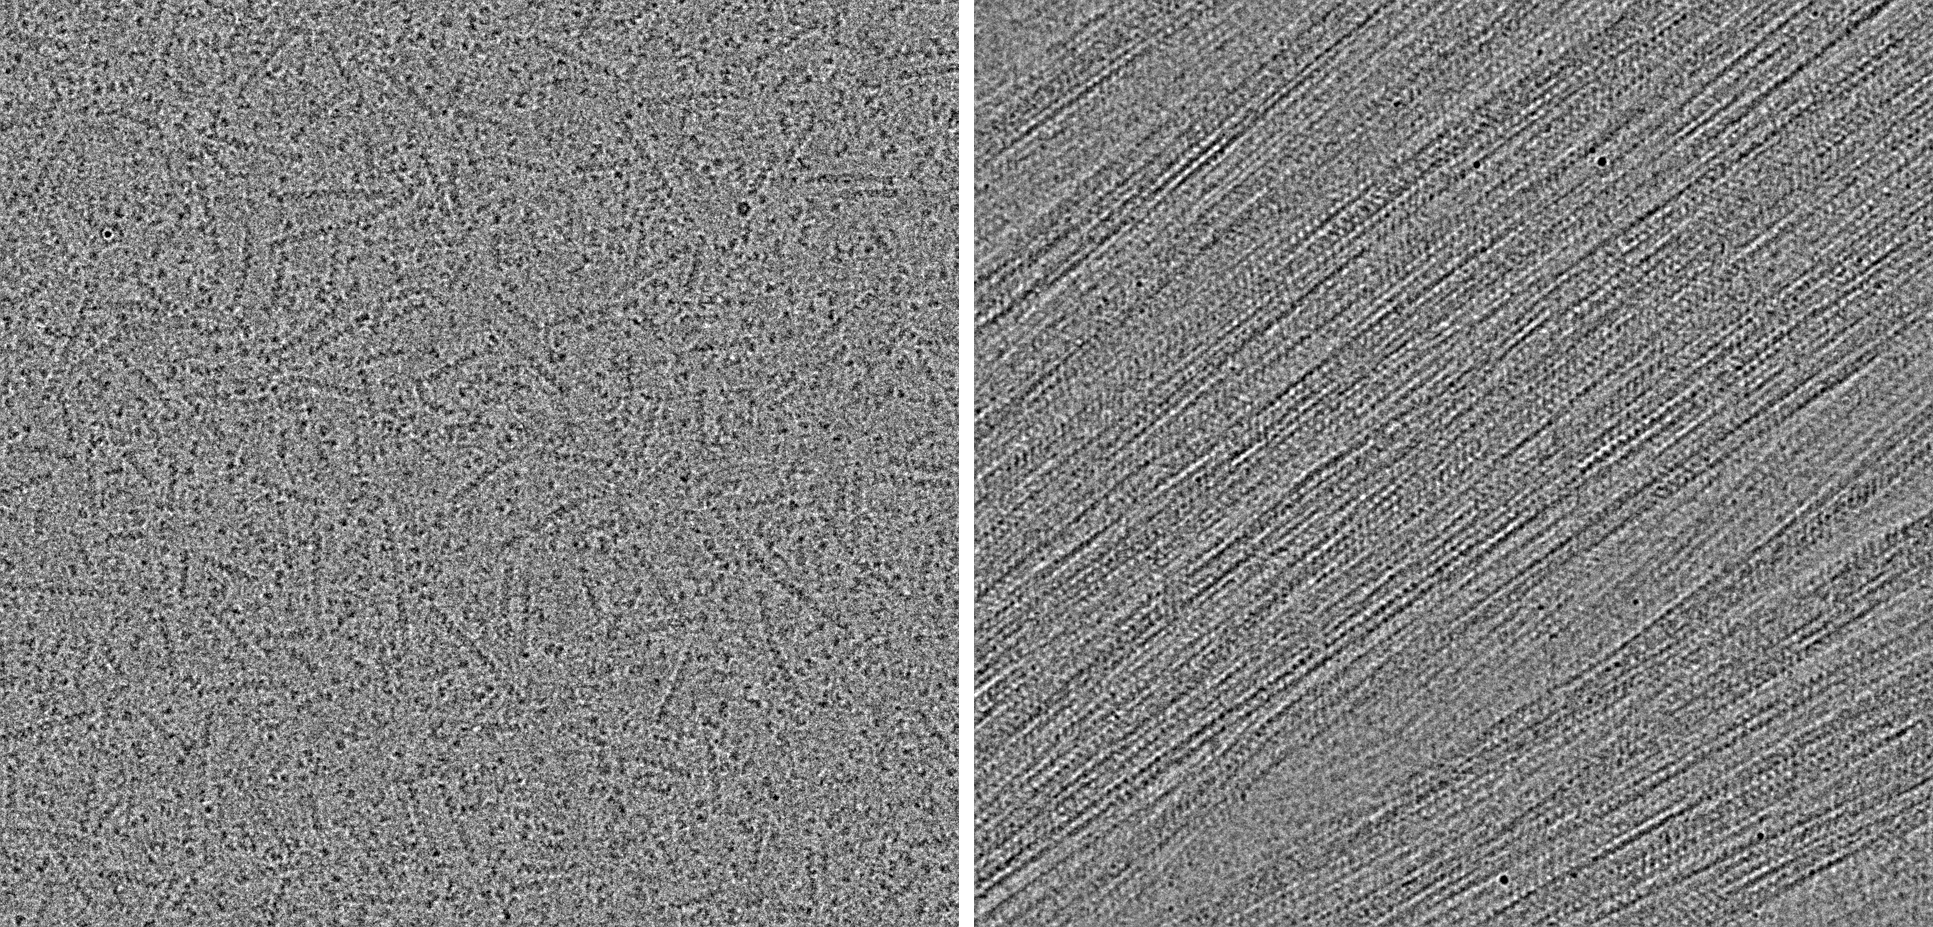
\includegraphics[width=\textwidth]{other/ftsz_mics.png}
    \titledcaption[Micrographs of FtsZ filaments]{Micrographs containing FtsZ filaments. When filaments are individual and well separated (left) they are ideal for picking and refinement. In some cases, FtsZ filaments form bundles (right) which are harder to pick, refine and classify due to the overlapping particles.}
    \label{fig:ftsz_micrographs}
\end{figure}

% TODO: data collection...?
We used CryoSPARC~\cite{punjaniCryoSPARCAlgorithmsRapid2017} for filament picking, which gave us a large amount of particles (>4M) to classify and clean up from spurious picks.
After cleaning, we ended up with about 2M particles, and very uniform classes with little variation (\autoref{fig:ftsz_classes}).
This is a typical symptom of strong preferential orientation due to the air-water interface (\fullref{em_pref_ori}), leading to a very limited range of views in the particle projections.
Though we saw hints of different views in the bundled filaments, they proved impossible to disentangle enough to obtain well-resolved classes.

\begin{figure}[ht]
    \centering
    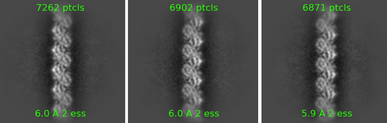
\includegraphics[width=\textwidth]{other/ftsz_classes_untilted.png}
    \titledcaption[FtsZ filament: 2D classes]{Classification results from particles with strong preferential orientation. All classes show very similar views of the FtsZ filaments, with minor variation in the out-of-plane angle.}
    \label{fig:ftsz_classes}
\end{figure}

Given the strong preferential orientation, it's unsurprising that 3D reconstructions from these particles showed very strong resolution anisotropy (while reporting \sim4 Å global resolution), so much so that we couldn't convincingly fit the monomeric model in the map (\autoref{fig:ftsz_map_bad}).

\begin{figure}[ht]
    \centering
    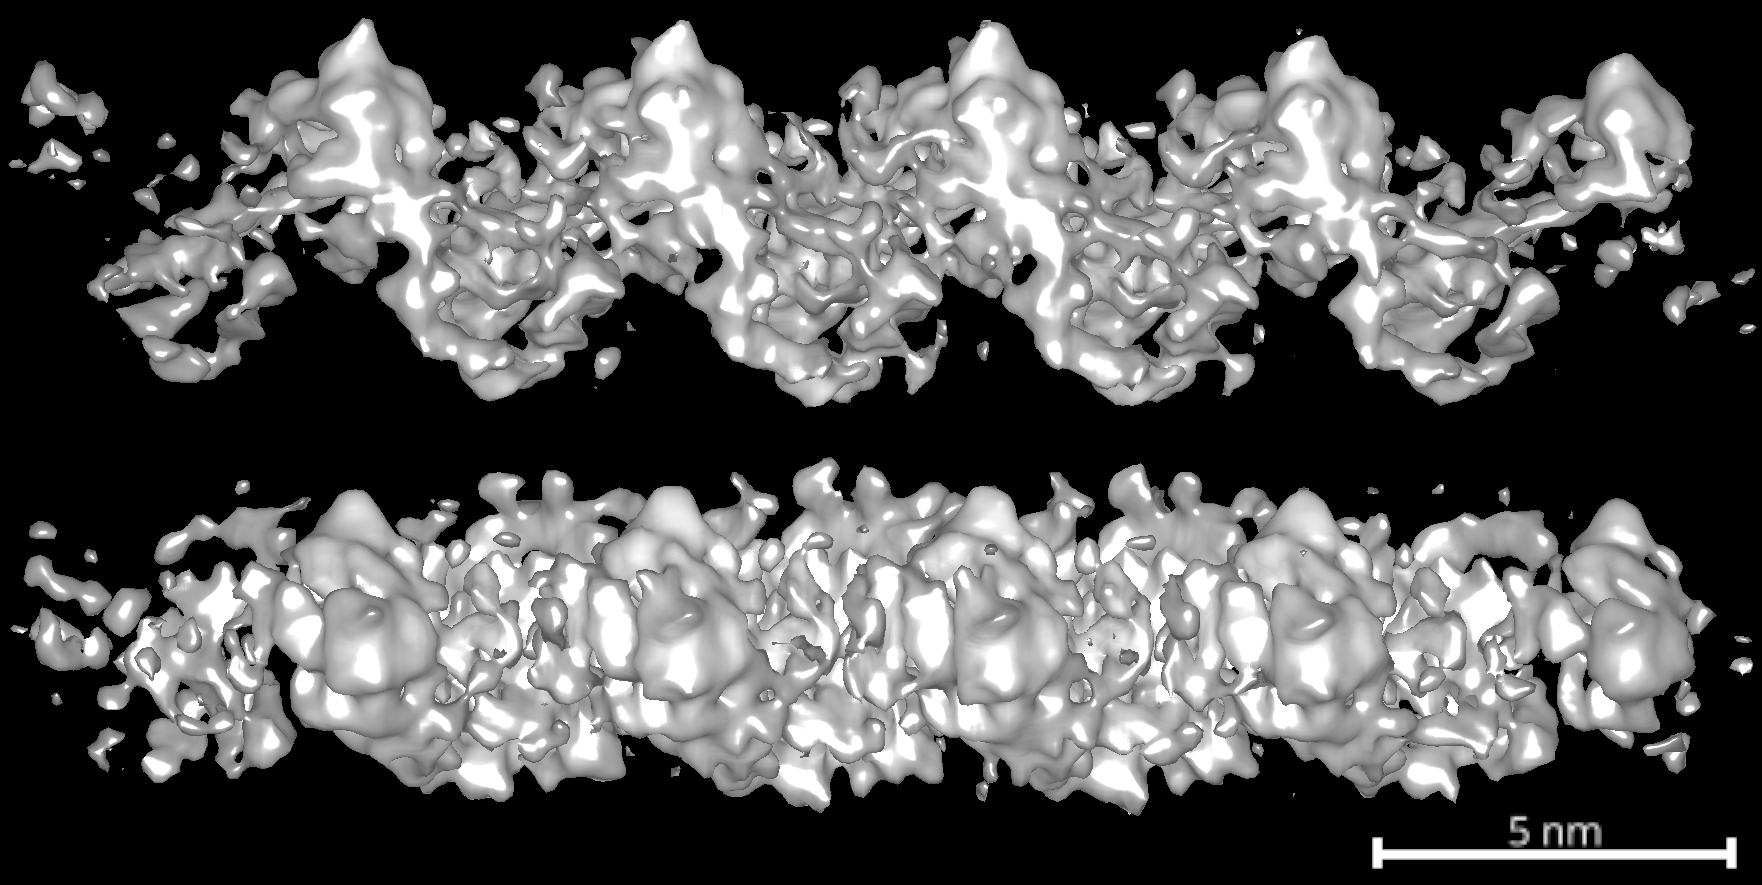
\includegraphics[width=\textwidth]{other/ftsz_map_bad.png}
    \titledcaption[FtsZ filament: anisotropic map]{FtsZ filament map affected by preferential orientation, viewed from the same direction as most 2D classes (top) and rotated by 90° (bottom) to highlight the streaking artifacts due to anisotropic orientation sampling.}
    \label{fig:ftsz_map_bad}
    % TODO: add pref orientation proof (orientation map or so)
\end{figure}

The best map currently available of FtsZ filaments (from \textit{Klebsiella pneumoniae}) also suffered from similar issues, despite the high reported resolution (\sim3 Å)~\cite{fujitaStructuresFtsZSingle2023}.

We attempted to address the issue of preferential orientation in two different ways: collecting a tilted dataset of the same samples, and preparing a new sample with methods that combat air-water interface effects.

\subsection{Graphene and streptavidin-coated grids}

We attempted to address the preferential orientation problem by using functionalized graphene grids~\cite{luFunctionalizedGrapheneGrids2022}, and streptavidin-coated affinity support grids~\cite{crucifixImmobilizationBiotinylatedDNA2004,hanLongShelflifeStreptavidin2016}.
While these approaches have been shown to work, we struggled to obtain usable grids; in the meantime, the sample prepared with the addition of detergent showed promising results, so we moved forward with it instead.

\subsection{Tilted data collection}\label{ftsz_tilted}

We prepared the sample in the same way, but this time the data collection was done with a 35° tilt.
Following the same workflow as with the untilted dataset, we then picked, classified and selected particles, obtaining a more promising selection of class averages (\autoref{fig:ftsz_classes_tilted}). % TODO: explain why these classes where better, did we get more, explain figure, what we were looking for, etc

\begin{figure}[ht]
    \centering
    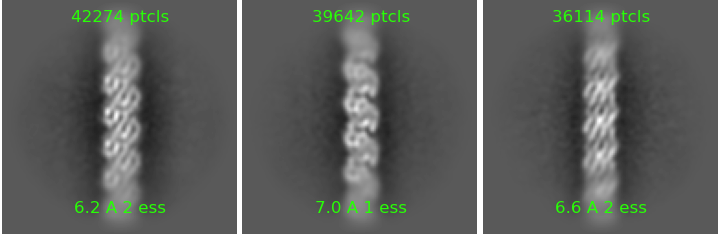
\includegraphics[width=\textwidth]{other/ftsz_classes_tilted.png}
    \titledcaption[FtsZ tilted dataset: 2D classes]{Classification results from the tilted dataset. Differently from the untilted classes, particles successfully classified into distinct views of the filament.}
    \label{fig:ftsz_classes_tilted}
\end{figure}

Despite the better view distribution of 2D classes, our 3D reconstructions had the same anisotropy issues as the untilted data.
Assuming a unform distribution of in-plane angles of the filaments (which we observed in the original dataset), a single, relatively high-tilt dataset should cover a higher portion of 3D fourier space during backprojection and thus significantly improve map isotropy~\cite{tanAddressingPreferredSpecimen2017}.

With preferentially oriented filaments collected at a fixed tilt angle, there should be a strong correlation between in-plane angle (easily identifiable from the micrograph) and the projection view (which is identified by classification). % TODO: show with synthetic dataset? Also, could it be that multiple euler combinations are redundant and correlation was just bad? How did I do this thing again?
Upon closer inspection of the picking data, however, we observed that the out-of-plane angles assigned to each particle showed no correlation with the assigned 2D class (\autoref{fig:ftsz_class_angles}).

\begin{figure}[ht]
    \centering
    \includegraphics[width=.5\textwidth]{example-image.png}
    \titledcaption{Out-of-plane angle plotted against the assigned 2D class. TODO}
    \label{fig:ftsz_class_angles}
\end{figure}

We soon realized that the 3D reconstruction routines of both Relion and CryoSPARC were struggling with assigning orientations, resulting in practically random orientations.
To impose more constraints on the refinement based on this prior knowledge on the geometry of the system, we calculated the theoretical orientation of each particle based on the in-plane angle (and assuming perfect preferential orientation), which we then used to initialize the particle poses (\fullref{stemia_angles}).

Unfortunately, this approach did not yet bear fruits: CryoSPARC does not provide fine control over angle priors and search patterns, and Relion parameter selection .... TODO (\autoref{fig:ftsz_angle_dist}).

\begin{figure}[ht]
    \centering
    \includegraphics[width=.5\textwidth]{example-image.png}
    \titledcaption{TODO: angle distribution plot}
    \label{fig:ftsz_angle_dist}
\end{figure}

\subsection{Addition of detergent}

Detergent has long been used as a way to address preferential orientation and aggregation of proteins in the sample.
In our case, while it did not affect the orientation problem, it allowed FtsZ to polymerize into longer filaments without creating large bundles (\autoref{fig:ftsz_ddm_mics}).

\begin{figure}[ht]
    \centering
    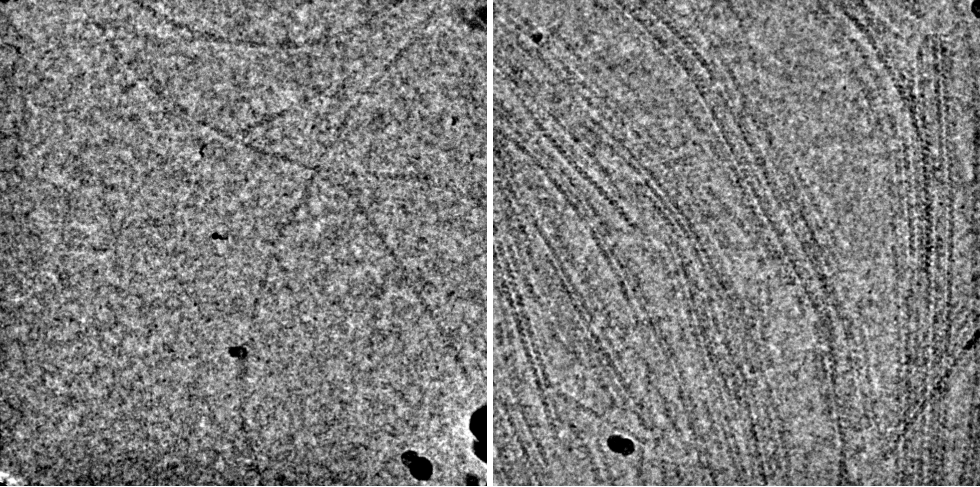
\includegraphics[width=.5\textwidth]{other/ftsz_mics_ddm.png}
    \titledcaption[Micrographs of FtsZ with detergent]{The addition of detergent allowed the FtsZ filaments to elongate further, without resulting in dense bundles (left). When bundles formed (right), they were often less densely packed than without detergent, opening up the possibility to pick bundled filaments in order to investigate side interactions.}
    \label{fig:ftsz_ddm_mics}
\end{figure}

The longer filaments and the very small helical twist (estimated at <1° with the previous samples), should result in different side views of the monomers being visible in the dataset.
Indeed, we observe a higher diversity in classification results, including classes with two or three filaments interacting side-by-side (\autoref{fig:ftsz_ddm_classes}).

\begin{figure}[ht]
    \centering
    \includegraphics[width=.5\textwidth]{example-image.png}
    \caption{TODO: ftsz ddm classes}
    \label{fig:ftsz_ddm_classes}
\end{figure}

Preliminary data showed an improvement in the map interpretability, although the anisotropy due to preferential orientation is still present (\autoref{fig:ftsz_ddm_map}).

\begin{figure}[ht]
    \centering
    \includegraphics[width=.5\textwidth]{example-image.png}
    \caption{TODO: my best ftsz map so far}
    \label{fig:ftsz_ddm_map}
\end{figure}

This project has now been taken over by Harald Bernhard, a postdoc in the MICA group, who managed to further improve the resolution by careful use of 3D classification to better separate single filaments from bundles, as well as... TODO


\section{Tomography and STA}

In parallel to the study of \textit{in vitro} FtsZ filament by SPA, we also investigated the FtsZ \textit{in situ} in the tomograms of \textit{D. radiodurans} lamellae.
Some of our findings and speculations about the 3D morphology of FtsZ are included in the \textit{D. radiodurans} manuscript (\fullref{drad_ftsz} and \fullref{ftsz_discussion}).

Our observations on the reconstructed tomograms matched those by \citet{sextonSuperresolutionConfocalCryoCLEM2022}, who also used tomography to look into D.rad and identified FtsZ and FtsA forming filaments just below the inner membrane of the septal tips (\autoref{fig:ftsz_tomo_slice}). % TODO: show more examples of this, how many have it, etc...

\begin{figure}[ht]
    \centering
    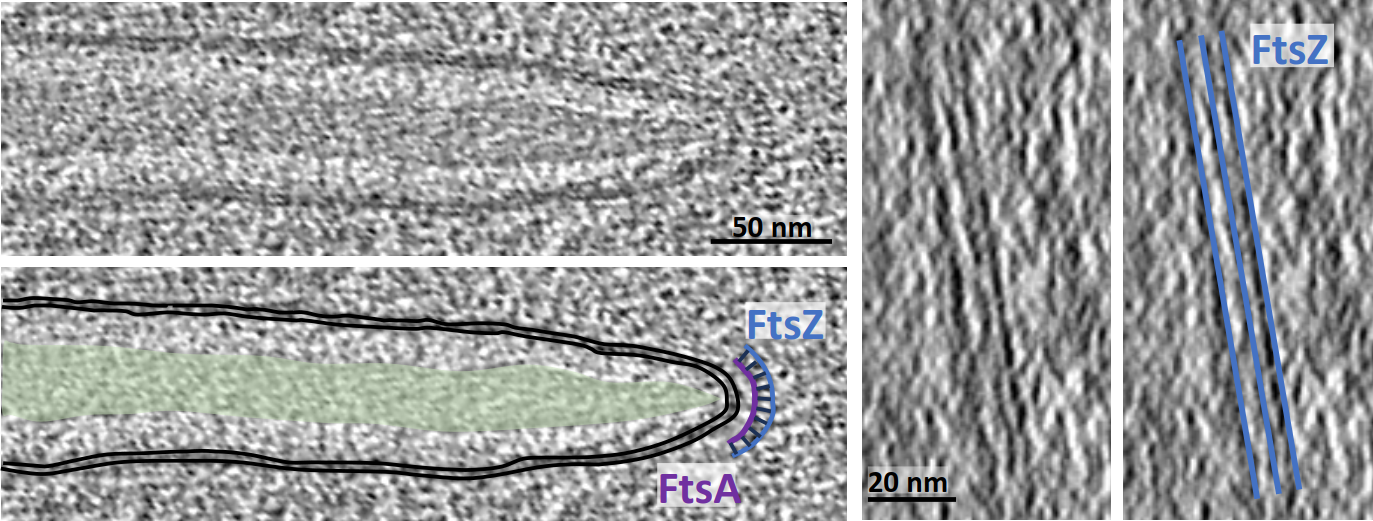
\includegraphics[width=.5\textwidth]{other/ftsz_slices.png}
    \titledcaption[FtsZ: tomogram slices from top and side view]{When viewing a cross-section of the bundle at the tip of the septa of \textit{D. radiodurans} (left), FtsZ is visible as a double arch separated by a gridded pattern. This is likely the result of a layer of FtsA bridging between the membrane and a layer of FtsZ filaments. (figure adapted from \autoref{ftsz_fig4}).}
    \label{fig:ftsz_tomo_slice}
\end{figure}

The size and spacing between FtsZ filaments is consistent with crystal structures and SPA studies on FtsZ filaments CITE.

The distance between FtsZ+FtsA filaments and the membrane in our tomograms is TODO, consistent with the expected \sim13-16~\cite{mcquillenInsightsStructureFunction2020}.
However, the width of the bundle appears to be smaller than the previously found 80-100 nm~\cite{mcquillenInsightsStructureFunction2020}, typically no wider than around 50-60 nm; this might be caused by differences in the thickess of the septa or modes of septation between different bacteria.
% TODO: double check

\subsection{Subtomogram averaging}

While it is clear that FtsZ and FtsA are forming filaments and bundles in vitro, and that they localize to the Z-ring in a bundle-like fashion, the details of this superstructural assembly are unknown.
To get a higher resolution view of this complex \textit{in situ}, we performed STA on particles picked from the FtsZ arches at the tips of the septa (\autoref{fig:ftsz_tomo_slice}).

Given the apparent regularity of the bundles (whose morphology appears unchanged across their length), we used blik's surface picking tool~\cite{gaifasBlikExtensible3D2024,gaifasBlikPythonTool2024}, which allows us to distribute regularly spaced particles on the sheet-like FtsZ bundles (\autoref{fig:ftsz_tomo_picks_surface}).
The inter-particle distance was chosen based on the smallest distance in the regular comb-like dark/light pattern along the FtsZ arches. % TODO: how many particles?
Two different sets of particles were thus generated: with exact inter-particle distance, and twice oversampled  (\autoref{fig:ftsz_tomo_picks_particles}).

\begin{figure}[ht]
    \centering
    \begin{subfigure}[B]{.5\textwidth}
        \centering
        \includegraphics[width=\textwidth]{example-image.png}
        \caption{TODO: surface of ftsz sheet}
        \label{fig:ftsz_tomo_picks_surface}
    \end{subfigure}%
    \hfill
    \begin{subfigure}[B]{.5\textwidth}
        \centering
        \includegraphics[width=\textwidth]{example-image.png}
        \caption{TODO: particle picks}
        \label{fig:ftsz_tomo_picks_particles}
    \end{subfigure}%
    \caption{TODO: surface picked with blik and particles generated on it (different spacings)}
    \label{fig:ftsz_tomo_picks}
\end{figure}

TODO

\section{Discussion and future perspectives}

Ice thickness should be negligible if we do proper CTF and motion correction (iteratively)~\cite{aiyerOvercomingResolutionAttenuation2024}.

We encountered a major obstacle in the preferential orientation of filaments both in SPA and STA; the project is still ongoing and the new detergent data is currently being processed.

\section{Materials and Methods}\label{ftsz_methods}

\subsection{Sample preparation for SPA}

\subsubsection{FtsZ only}
5μl FtsZ at 12.5 mg/ml were diluted in 4 μl buffer (50 mM Tris-HCl pH 8.0, 200 mM NaCl), and 1 μl GpCpp at 10 mM.
Mix was then incubated at 25°C for 75 min to allow for filament elongation.
4μl of mix was then diluted in 16 μl of buffer (50 mM Tris-HCl pH 8.0, 200 mM NaCl), and 1 μl GpCpp at 10 mM.
The sample was then immediately frozen on R2/1 300mesh EM grids (blot time: 3.5 s).

\subsubsection{FtsZ+DDM}
2μl FtsZ at 12.5 mg/ml were diluted in 16 μl buffer (50 mM Tris-HCl pH 8.0, 200 mM NaCl), and 2 μl GpCpp at 10 mM.
Mix was then incubated at 25°C for 30 min to allow for filament elongation, after which 2μl DDM at 0.09\% was added.
Grids were frozen with and without further 5x dilution in buffer (50 mM Tris-HCl pH 8.0, 200 mM NaCl, 1 mM GpCpp, 0.009\% DDM: 2 μl mix + 8 μl buffer)

TODO: should we include details about reproducibility/elongation? I added some to the text above, but maybe we need more details here.

TODO: graphene and streptavidin grids

\subsection{Data Collection for SPA}

TODO: I need help here for the technical microscopy details...

\subsection{SPA processing}

filament picking (parameters, issues with length)

link to \fullref{stemia_angles}.

\subsection{\textit{D. radiodurans} lamellae and tomography data collection}

See \fullref{drad_lamellae_method} and \fullref{drad_tomo_method}.

\subsection{STA data processing}

blik, relion
